%% Settings for single-side (simplex) printing
% Margins: left 40mm, right 25mm, top and bottom 25mm
% (but beware, LaTeX adds 1in implicitly)
\documentclass[12pt,a4paper]{report}
\setlength\textwidth{145mm}

\usepackage[utf8]{inputenc}
\usepackage{graphicx}
\usepackage{fancyhdr}
\usepackage{lmodern}
\usepackage{lastpage}
\usepackage{subfig}

\graphicspath{{../graphs/}}

\pagestyle{fancy}
\fancyhf{}
\rhead{Petr Houška `houskape@gmail.com`}
\lhead{HW2: Fibonacci heap}
\rfoot{Page \thepage / \pageref{LastPage}}


\begin{document}
	
	
	\begin{figure}[h]	
		\centering	
		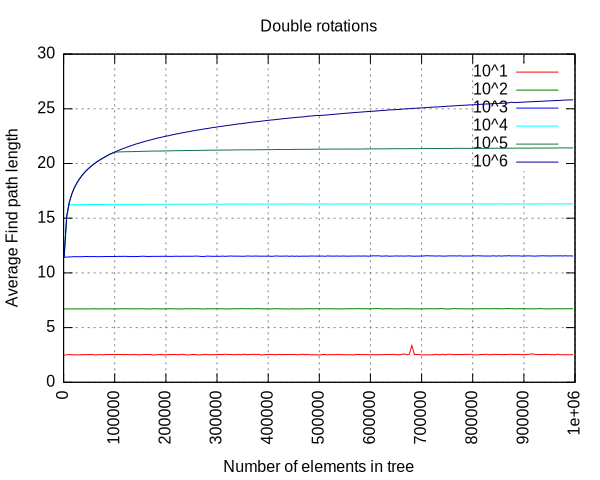
\includegraphics[scale=1]{graph_1}		
	\end{figure}

	\begin{figure}[h]	
    \centering
		\subfloat{{\includegraphics[scale=0.5]{graph_1_1}	 }}%
		\qquad
		\subfloat{{\includegraphics[scale=0.5]{graph_1_2}	}}%
    \end{figure}



Lorem Ipsum.

	\begin{figure}[h]	
		\centering	
		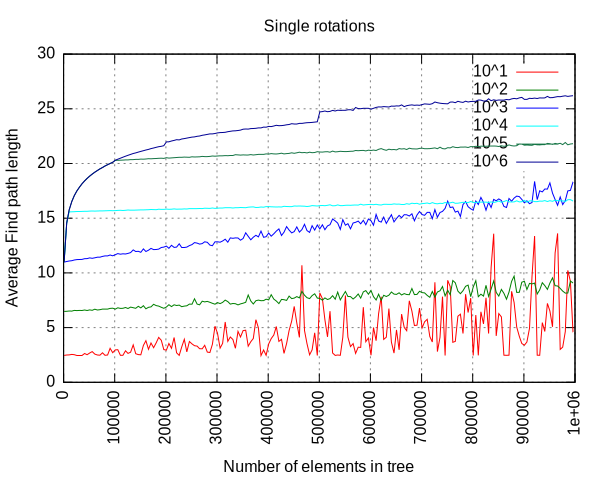
\includegraphics[scale=1]{graph_2}		
	\end{figure}

Lorem Ipsum.


\end{document}